\documentclass{article}

\textwidth=6.5in
\textheight=8.5in
\voffset=-54pt
\oddsidemargin=0in
\evensidemargin=0in
\setlength{\parskip}{8pt}
\setlength{\parindent}{0pt}

\usepackage{amsmath, amssymb}
\usepackage{ifthen}

\usepackage[inline]{enumitem}
\setlist{topsep=0pt, parsep=8pt}

\usepackage[rgb,table]{xcolor}\convertcolorsUfalse
\usepackage{graphicx}

% change hyperref options
\PassOptionsToPackage{hyphens}{url}
\usepackage[bookmarks,colorlinks,linkcolor=black,citecolor=blue,pdfstartview=FitH,urlcolor=blue]{hyperref}
\hypersetup{pdfpagemode=UseNone}
\usepackage{bookmark}

\usepackage{graphicx}
\usepackage{multicol}
\usepackage{framed}
\usepackage{array}

\usepackage{icomma}

\usepackage{soul}

\usepackage{pgfplots}
\pgfplotsset{compat=1.18}  
\pgfplotscreateplotcyclelist{mycolor}{black, blue, red, green!70!black, magenta, purple, cyan, orange }  
\pgfplotsset{
  disabledatascaling,
  cycle list=tikzcolor, 
  axis lines=middle,
  every axis plot/.style={no marks, thick},
  every axis/.style={
    enlarge x limits=false,
    enlarge y limits=auto,
    xlabel style={at={(current axis.right of origin)},anchor=west},
    ylabel style={at={(current axis.above origin)},anchor=south},
    % extra x and y ticks for asymptotes
    extra x tick style={grid=major, grid style={dashed,black}},
    extra y tick style={grid=major, grid style={dashed,black}},
    /pgf/number format/1000 sep={},
  },    
  tick label style = {font=\footnotesize, fill=\currentbgcolor, inner sep=0pt},    
  xticklabel shift=1pt,    
  scaled ticks=false,
  scaled y ticks=false,
  unbounded coords=jump,
  samples=101,
  minor tick length=0,
  scatter/classes={
    open={mark=*,draw=black,fill=white, mark size=2, thin},
    closed={mark=*,draw=black,fill=black, mark size=2, thin}
  },
  width=3in,
}
\pgfplotsset{open/.style={only marks, mark=*, fill=white, thin, mark size=2}}
\pgfplotsset{closed/.style={only marks, mark=*, draw=black, fill=black,
    thin, mark size=2}}
\pgfplotsset{labeled/.style={nodes near coords, only marks, mark=*, draw=black, fill=black, thin, mark size=2, point meta=explicit symbolic}}

\pgfplotsset{gridgraph/.style={clip=false, axis line style={shorten
      >=-8pt}, xlabel style={xshift=8pt}, ylabel style={yshift=8pt},
    enlargelimits=false, grid=major, tick style={black}}} 

\newcommand{\axes}[1][]{
  \begin{tikzpicture}
    \begin{axis}[xtick=\empty, ytick=\empty, ymin=-2, ymax=2,
      xmin=-4.25, xmax=4.25, #1]
    \end{axis}
  \end{tikzpicture}
}
\usepackage{tikz}
\usetikzlibrary{
  matrix,%
  % enables the snake paths
  decorations.pathmorphing,%
  % enables bigger arrows
  decorations.markings,%
  decorations.pathreplacing,%
  decorations.text,%
  calc,%
  patterns,%
  shapes.geometric,%
  arrows,
  decorations.shapes,
  positioning,
  plotmarks,
  intersections
}
\tikzset{>=latex} % sets default arrow type in tikz
\tikzset{font=\normalsize}
\tikzset{mark size=1.5pt, mark options=thin}
\tikzset{pin distance=4pt,
  every pin edge/.style={<-, thin, shorten <= -2pt}}

\interfootnotelinepenalty=10000
\renewcommand{\thefootnote}{(\arabic{footnote})}

\usepackage{multirow, bigdelim}

% change to \usepackage[sols]{handout} to see solutions
\usepackage[]{handout}

\newcommand\iscurrentenumi[1]{%
  \ifthenelse{\equal{#1}{\theenumi}}{}{#1}}
\setenumerate[1]{ref=\#\arabic*}
\setenumerate[2]{ref=\protect\iscurrentenumi{\theenumi}(\alph*)}
\newcommand\enumiiprefix[2]{%
  \ifthenelse{{\equal{#1}{\theenumi}}\AND{\equal{#2}{(\alph{enumii})}}}{}{}%
  \ifthenelse{{\equal{#1}{\theenumi}}\AND{\NOT{\equal{#2}{(\alph{enumii})}}}}{#2}{}%
  \ifthenelse{\equal{#1}{\theenumi}}{}{#1#2}%
}
\setenumerate[3]{ref=\protect\enumiiprefix{\theenumi}{(\alph{enumii})}\roman*}

\makeatletter

\newdimen\SOUL@dimen %new
\def\SOUL@ulunderline#1{{%
    \setbox\z@\hbox{#1}%
    % \dimen@=\wd\z@
    \SOUL@dimen=\wd\z@ %new
    \dimen@i=\SOUL@uloverlap
    \advance\SOUL@dimen2\dimen@i %\dimen@ exchanged too
    \rlap{%
      \null
      \kern-\dimen@i
      % \SOUL@ulcolor{\SOUL@ulleaders\hskip\dimen@}%
      \SOUL@ulcolor{\SOUL@ulleaders\hskip\SOUL@dimen}% new
    }%
    \unhcopy\z@
  }}

\makeatother

\definecolor{purple}{rgb}{0.5,0,1.0}

\usepackage{fancyhdr}
\lhead{\textcolor{white}{This content is protected and may not be shared, uploaded, or distributed.}}
\rhead{}
\rfoot{\vspace*{\fill}\footnotesize\textcopyright{} \emph{Harvard Math Ma}}
\renewcommand{\headrulewidth}{0pt}
\pagestyle{fancy}
\begin{document}

\htitle{Exam 1 Practice}

\begin{enumerate}
\item  \label{stretching-derivatives}

  \begin{enumerate}
  \item

    \note{Just by looking at the graph, we can see that the slope is positive and greater than 10.}

    \begin{problem}[\vfill]
      The picture in \ref{stretching-derivatives-vertical} shows the graph of a function $f$. One of these is the value of $f'(-1)$; which one? Explain how you can eliminate the other choices.
      \[ -18 \qquad -3 \qquad 3 \qquad 18 \]
    \end{problem}

    \begin{solution}
      $f'(-1)$ is the slope of the tangent line to the graph of $y=f(x)$ at $x=-1$.
      Looking at the graph in \ref{stretching-derivatives-vertical}, we can see
      that the slope of the tangent line at $x=-1$ is positive, so we can eliminate
      $-3$ and $-18$. 

      \begin{tikzpicture}
        \begin{axis}[xtick={-1, 2, 5}, ytick={10}, clip=false, width=2.75in]
          \addplot+[domain=-2:6] {(x + 1)*(x-2)*(x-5)} node[right]{$y = f(x)$};
          \addplot[domain=-2:0, red] {18*(x+1)};
          \addplot[domain=-2:1, blue] {10*(x+1)};
        \end{axis}
      \end{tikzpicture}
      
      To decide between $3$ and $18$, we need to be able to say something about
      the steepness of the tangent line. Looking at the graph, the tangent line at $x=-1$, shown in red, is steeper than the secant
      line between $x=-1$ and $x=0$, shown in blue. 
      The secant line has a slope of $10$, so
      we can eliminate $3$ as an option. This leaves $f'(-1)=18$.
    \end{solution}

  \end{enumerate}
  This table shows some additional values of $f'$:
  \begin{center}
    \begin{tabular}{c | r r r r r r}
      $x$ & 0 & 1 & 2 & 3 & 4 \\
      \hline
      $f'(x)$ & $3$ & $-6$ & $-9$ & $-6$ & $3$
    \end{tabular}
  \end{center}
  \begin{enumerate}[resume, topsep=0pt]
  \item \label{stretching-derivatives-vertical}
    \begin{problem}
      On the axes below, sketch the graph of $g(x) = 2 f(x)$, and label any intercepts.

      \begin{tikzpicture}
        \begin{axis}[xtick={-1, 2, 5}, ytick={10,\solonly{20}}, clip=false,
        width=2.75in, restrict y to domain=-30:30]
          \addplot+[domain=-2:6] {(x + 1)*(x-2)*(x-5)} node[right]{$y = f(x)$};
          \solonly{
          \addplot[domain=-1.5:-0.5] {18*(x+1)};
          \addplot[domain=-1.5:-0.5, red] {36*(x+1)};
          \addplot+[domain=-2:6, red] {2*(x + 1)*(x-2)*(x-5)} node[left]{$y = 2f(x)$};
          }
        \end{axis}
      \end{tikzpicture}
    \end{problem}

  \item
    \begin{problem}[\vfill]
      What's $g'(-1)$? Explain. 
    \end{problem}

    \begin{solution}
      The graph of $y=g(x)$ is the graph of $y=f(x)$ but scaled by a factor of 2
      in the vertical direction. 
      This means that the line tangent to the graph at $x=-1$ would
      also be scaled by a factor of 2 in the vertical direction, so the slope of
      the tangent line would be 36. Therefore $g'(-1)=36$.
    \end{solution}

  \item

    \begin{problem}
      Here's the graph of $f$ again. On the same axes, sketch the graph of $h(x) = f(2x)$, and label any intercepts.

      \begin{tikzpicture}
        \begin{axis}[xtick={-1, 2, 5, \solonly{-0.5,1,2.5}},
        ytick={10}, clip=false, width=2.75in, 
        xticklabels={$-1$,$2$,$5$,\solonly{$\frac{-1}{2}$},\solonly{$1$},
        \solonly{$\frac{5}{2}$}}]
          \addplot+[domain=-2:6] {(x + 1)*(x-2)*(x-5)} node[right]{$y = f(x)$};
          \solonly{
          \addplot[domain=1:3] {-9*(x-2)};
          \addplot[domain=0.5:1.5, red] {-18*(x-1)};
          \addplot+[domain=-1:3, red] {(2*x + 1)*(2*x-2)*(2*x-5)} node[right]{$y = f(2x)$};
          }
        \end{axis}
      \end{tikzpicture}
    \end{problem}

  \item

    \note{We'll eventually use this idea to find the derivative of $e^{kx}$.}

    \begin{problem}[\vfill\newpage]
      What's $h'(1)$? Explain.
    \end{problem}

    \begin{solution}
      The graph of $y=h(x)$ is the graph of $y=f(x)$ but scaled by a factor of
      $\frac{1}{2}$ in the horizontal direction. 
      This means the line tangent to the graph of $y=h(x)$
      at $x=1$ would be a rescaled version of the line tangent to the
      graph of $y=f(x)$ at $x=2$. The slope of the rescaled line
      would be twice the slope of the original line. Since $f'(2)=-9$,  
      this means that $h'(2)=-18$. 
    \end{solution}
  \end{enumerate}

\item  \label{fall2018-final-practice4-2}

  Here's the graph of a function $f$ on $(-5, 3)$:
  \begin{center} 
    \begin{tikzpicture}
      \begin{axis}[xtick={-5, -4, ..., 3}]
        \addplot+[domain=-5:-2] {1/(2*x+3) +1};  
        \addplot+[domain=-2:3]{-.5*x^2+2};
      \end{axis}
    \end{tikzpicture}
  \end{center}

  \begin{enumerate} 
  \item
    \begin{problem}[\vfill]
      Sketch a graph of $f'$.
    \end{problem}

    \begin{solution}
      Here's the graph:
      \begin{center} 
        \begin{tikzpicture}
          \begin{axis}[xtick={-5, -4, ..., 3}]
            \addplot+[domain=-5:-2] {-2/(2*x+3)^2 }; %
            \addplot+[domain=-2:3]{-x}; %
            \addplot[open] coordinates{(-2, -2)}; %
            \addplot[open] coordinates{(-2, 2)}; %
          \end{axis}
        \end{tikzpicture}
      \end{center}       

      Note: Your graph should be decreasing when $x > -2$, and it should pass through the origin, but it's okay if it isn't linear. We don't have enough information to be sure of whether that piece is linear.
    \end{solution}

  \end{enumerate}

  Now, suppose $g$ is a function such that $g'(x) = f(x)$.

  \begin{enumerate}[resume]
  \item

    \note{For increasing, both $(-5, -2) \cup (-2, 2)$ and $(-5, 2)$ are okay.}

    \begin{problem}[\stretch{0.3}]
      Where on $(-5, 3)$ is $g$ increasing? Where on $(-5, 3)$ is $g$ decreasing?
    \end{problem}

    \begin{solution}
      $g$ will be increasing on intervals where $g'$ is positive. 
      Since $g'(x)=f(x)$, we can look at the graph of $y=f(x)$ to determine
      that $g'$ is positive on $(-5, -2) \cup (-2, 2)$. This means that $g$ is
      increasing on $(-5, 2)$.

      Since $g'$ is negative on $(2, 3)$, $g$ is decreasing on $(2, 3)$. 
      
    \end{solution}

  \item
    \begin{problem}[\stretch{0.3}]
      Where on $(-5, 3)$ is $g$ concave up? Where on $(-5, 3)$ is $g$ concave down? 
    \end{problem}

    \begin{solution}
      To determine where $g$ is concave up, we need to determine where $g''$ is
      positive. Since $g''(x) = f'(x)$, we can look at the graph we sketched of
      $y=f'(x)$ to determine that $g''$ is positive on $(-2, 0)$. Thus,
      $g$ is concave up on $(-2, 0)$. 

      Since $g''$ is negative on $(-5, -2) \cup (0, 3)$, we can say that
      $g$ is concave down on $(-5, -2)$ and $(0, 3)$. 
    \end{solution}

  \item
    \begin{problem}[\newpage]
      What's $g'(-2)$?
    \end{problem}

    \begin{solution}
        $g'(-2) = f(-2) = 0$. 
    \end{solution}

  \item

    \note{As usual, the main point is consistency with the previous parts.} 

    \begin{problem}
      If $g(0) = 1$, sketch a graph of $g$ on the axes below.
    \end{problem}

    \begin{problemonly}
      \axes[xmin=-5, xmax=3, xtick={-5, -4, ..., 3}, width=3.5in]
    \end{problemonly} 

    \begin{solution}
      We know that
      \begin{itemize}
        \item $g$ is increasing on $(-5, 2)$
        \item $g$ is decreasing on $(2, 3)$
        \item $g$ has a horizontal tangent at $x=-2$
        \item $g$ is concave up on $(-2, 0)$
        \item $g$ is concave down on $(-5, 2)$ and $(0, 3)$
        \item $g$ has a $y$-intercept at $(0,1)$
      \end{itemize}
      Based on this information, we can sketch the graph of $g$.
      
      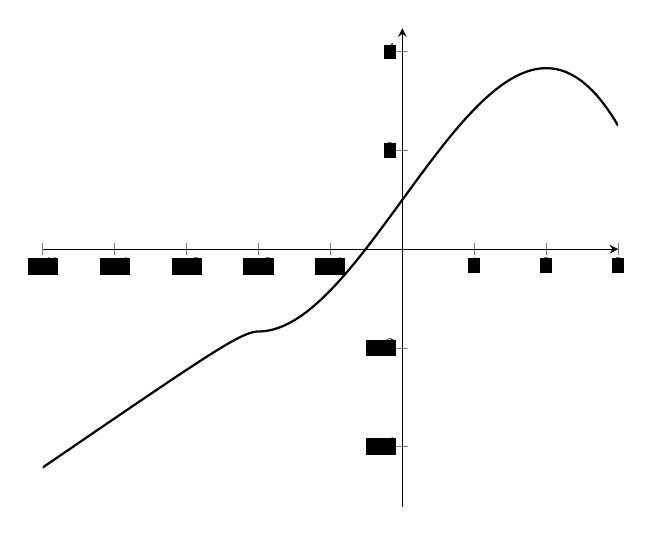
\begin{tikzpicture}
        \begin{axis}[xmin=-5, xmax=3, xtick={-5, -4, ..., 3}, width=3.5in]
          \addplot[domain=-5:-2] {-0.25/(2*x+3)^2 +x + 9/4 - 5/3};
          \addplot[domain=-2:3] {(-x^3)/6 + 2*x +1};
        \end{axis}
      \end{tikzpicture}
    \end{solution}


  \end{enumerate} 

  \pspace{\vfill}

\item  In each part, you're given the graph of a function $f$ and an expression. On the graph, sketch a line whose slope is the given expression.

  \begin{multicols}{2}
  \begin{enumerate}
  \item
    \begin{problem}
        $\dfrac{f(2 + h) - f(2)}{h}$ where $h = -0.5$
    \end{problem}

    \begin{tikzpicture}[
    declare function={f(\x) = cos(deg(1.8*\x^(0.9)))*1.1^\x;}
    ]
        \begin{axis}[gridgraph, ytick=\empty, ymin=-2, ymax=2, width=3.15in, height=2in]
        \addplot+[domain=0:5] {f(x)}; 
        \solonly{
        \addplot[domain=0:4, blue] {((f(1.5)-f(2))/(-0.5))*(x-2) + f(2)};
        }
      \end{axis}      
    \end{tikzpicture}

  \item
    \begin{problem}
        $\displaystyle \lim_{h \to 2} \dfrac{f(2 + h) - f(2)}{h}$
    \end{problem}

    \begin{tikzpicture}[
    declare function={f(\x) = cos(deg(1.8*\x^(0.9)))*1.1^\x;}
    ]
        \begin{axis}[gridgraph, ytick=\empty, ymin=-2, ymax=2, width=3.15in, height=2in]
        \addplot+[domain=0:5] {f(x)}; 
        \solonly{
        \addplot[domain=1.5:4.5, blue] {((f(4)-f(2))/(2))*(x-2) + f(2)};
        }
      \end{axis}      
    \end{tikzpicture}

    \end{enumerate}
  \end{multicols}

  \pspace{\vfill}

  \begin{enumerate}[start=3]
  \item
    \begin{problem}
        $\displaystyle \lim_{h \to 0} \dfrac{f(2 + h) - f(2)}{h}$
    \end{problem}

    \begin{tikzpicture}[
    declare function={f(\x) = cos(deg(1.8*\x^(0.9)))*1.1^\x;}
    ]
        \begin{axis}[gridgraph, ytick=\empty, ymin=-2, ymax=2, width=3.15in, height=2in]
        \addplot+[domain=0:5] {f(x)};
        \solonly{
        \addplot[domain=0:5, red] {((f(2.001)-f(2))/(0.001))*(x-2) + f(2)};
        }
      \end{axis}      
    \end{tikzpicture}

      \pspace{\vfill\newpage}
    \end{enumerate}

  \solonly{\newpage}

  \begin{multicols}{2}
    \begin{enumerate}[start=4]
  \item
    \begin{problem}
        $\dfrac{f(t) - f(3)}{t - 3}$ where $t = 1$
    \end{problem}

    \begin{tikzpicture}[
    declare function={f(\x) = cos(deg(1.8*\x^(0.9)))*1.1^\x;}
    ]
        \begin{axis}[gridgraph, ytick=\empty, ymin=-2, ymax=2, width=3.15in, height=2in]
        \addplot+[domain=0:5] {f(x)}; 
        \solonly{
        \addplot[domain=0:5, blue] {((f(1)-f(3))/(-2))*(x-3) + f(3)};
        }
      \end{axis}      
    \end{tikzpicture}

  \item
    \begin{problem}
        $\displaystyle \lim_{t \to 3} \dfrac{f(t) - f(3)}{t - 3}$
    \end{problem}

    \begin{tikzpicture}[
    declare function={f(\x) = cos(deg(1.8*\x^(0.9)))*1.1^\x;}
    ]
        \begin{axis}[gridgraph, ytick=\empty, ymin=-2, ymax=2, width=3.15in, height=2in]
        \addplot+[domain=0:5] {cos(deg(1.8*x^(0.9)))*1.1^x}; 
        \solonly{
        \addplot[domain=2:4, red] {((f(3.001)-f(3))/(0.001))*(x-3) + f(3)};
        }
      \end{axis}      
    \end{tikzpicture}

    \end{enumerate}
  \end{multicols}

  \pspace{0.25in}

\item  \label{fall2011-premidterm-1} 

  Harvard is building a new running track which is to be 400 meters long. It is to be the perimeter of a region obtained by putting two semicircles on opposite ends of a rectangle, as shown in the picture below (the track is the heavy dark line).

  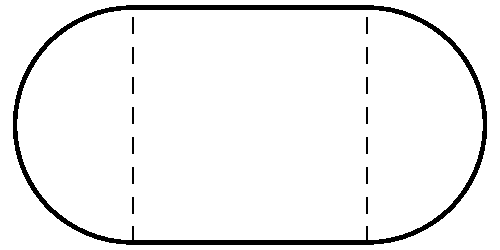
\includegraphics[width=2in]{images/modeling-track} 

  \begin{enumerate}
  \item \label{fall2011-premidterm-1-area}
    \begin{problem}[\vfill]
      Express the area enclosed by the track as a function of the radius of the ends.
    \end{problem}

    \begin{solution}
      The goal is to find an formula for the the area enclosed by the track as a function
      of the radius of the semicircular ends. We know that the running track
      is 400 meters long in total. Let's draw a picture to get a feel for
      the situation, and we'll define any variables we use.

      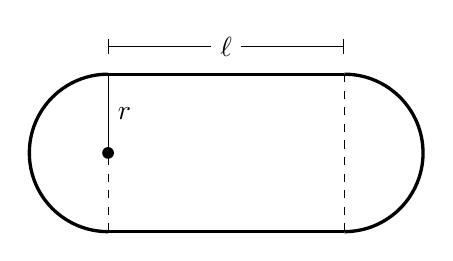
\begin{tikzpicture}
        \draw[very thick] (0,0) -- (3,0);
        \draw[very thick] (0,2) -- (3,2);
        \draw[dashed] (0,0) -- (0,2);
        \draw[dashed] (3,0) -- (3,2);
        \draw[very thick] (0,2) arc (90:270:1);
        \draw[very thick] (3,0) arc (-90:90:1);
        \draw[|-|, yshift=1em] (0,2) -- node[midway, fill=white]{$\ell$} (3, 2); 
        \node[circle, fill=black, inner sep=1.5pt] at (0,1) {};
        \draw (0,1) -- node[midway, right] {$r$} (0, 2);
      \end{tikzpicture}

      We'll call the length of one of the straight sides of the track $\ell$,
      and we'll call the radius of the semicircular ends $r$.

      Now let's write a formula for the area enclosed by the track, which we'll
      call $A$. First, we can write
      \begin{align*}
          A &= A_\text{circle} + A_\text{rectangle}, \\
          \intertext{where $A_\text{circle}$ is the area of enclosed
          by the two semicircular ends shown in our drawing and
          $A_\text{rectangle}$ is the area of the rectangular region.
          $A_\text{circle}$  is $\pi r^2$, and $A_\text{rectangle}$ is $2r\ell$, so}
          A &= \pi r^2 + 2r\ell. \\
          \intertext{Now, to express $\ell$ in terms of $r$, we need to use the information
          given in the problem. We know that the perimeter of the track is to be $400$
          meters, so $2\pi r + 2\ell = 400$. Solving this for $\ell$, we find that
          $\ell = 200 - \pi r$. We can then substitute this into our formula for the area
          to obtain $A$ as a function of $r$.}
          A &= \pi r^2 + 2r(200-\pi r) \\
          &= 400r - \pi r^2
      \end{align*}
    \end{solution}

  \item
    \begin{problem}[\nstretch{0.25}]
      What is the domain of the function in \ref{fall2011-premidterm-1-area}? 
    \end{problem}

    \begin{solution}
      To find the domain, we need to consider all possible values of $r$. The radius
      cannot be negative, but it could potentially be
      zero,\footnote{You could also argue that the radius can be very small
      but not exactly zero, so $r > 0$. Later on, we'll see why it's
      convenient to include the endpoints in our domain when possible.}
      in which case the track is just
      a straight line back and forth. This is the minimum value of $r$.
      
      There should be a maximum value of $r$,
      because the perimeter must be $400$ meters exactly, 
      so $r$ cannot be arbitrarily large. 
      When $r$ is large, $\ell$ must be small for the perimeter to be $400$ meters. 
      The maximum value of $r$ will therefore be when $\ell$ is as small as possible.
      The smallest possible value of $\ell$ is zero, and the maximum possible value of $r$
      is $\frac{200}{\pi}$.

      The domain is $0 \leq r \leq \frac{200}{\pi}$. ($0 < r < \frac{200}{\pi}$ would also be acceptable.)
    \end{solution}

  \item \label{fall2011-premidterm-1-cost}
    \begin{problem}[\vfill]
      The curved portions of the track will cost \$5 per meter to build, and the straight portions will cost \$3 per meter. Express the cost of the track as a function of the radius of the ends.
    \end{problem}

    \begin{solution}
      The goal is to write down the cost of building the track as a function of the radius
      of the ends. We know that the cost per length of the curved portions is \$5 per meter,
      and the cost per length of the straight portions is \$3 per meter. Since we've already
      drawn a picture, let's go ahead and come up with a formula for the cost. First,
      we can say
      \begin{align*}
        C &= C_\text{curved} + C_\text{straight} \\
        \intertext{where $C$ is the total cost, $C_\text{curved}$ is the cost of the 
        curved portions, and $C_\text{straight}$ is the cost of the straight portions.
        Letting $L_\text{curved}$ be the total length of the curved portions
        and $L_\text{straight}$ be the total length of the straight portions, we can write}
        C &= 5L_\text{curved} + 3L_\text{straight} \\
        &= 5(2\pi r) + 3(2\ell) \\
        &= 10\pi r + 6\ell \\
        \intertext{To write this as a function of $r$, we can use the relationship
        we found previously that $\ell = 200 - \pi r$.}
        C &= 10 \pi r + 6(200 - \pi r) \\
        &= 1200 + 4\pi r.
      \end{align*}
    \end{solution}

  \item
    \begin{problem}[\stretch{0.15}]
      What is the domain of the function in \ref{fall2011-premidterm-1-cost}? 
    \end{problem}

    \begin{solution}
      The domain of this function is the same as the domain of the previous function,
      $0 \leq r \leq \frac{200}{\pi}$.
      ($0 < r < \frac{200}{\pi}$ would also be acceptable.) 
    \end{solution}

  \end{enumerate}

\item 
  Let $f(x) = 3 + \dfrac{1}{x - 2}$.

  \begin{enumerate}
  \item
    \begin{problem}[\nstretch{1.5}]
      Use the definition of the derivative to calculate $f'(1)$. 
    \end{problem}

    \begin{solution}
      First, let's write down the definition of the derivative. 
      \begin{align*}
        f'(1) &= \lim_{h \to 0} \frac{f(1+h)-f(1)}{h} \\
        &= \lim_{h \to 0} \frac{3 + \frac{1}{1+h-2} - 2}{h} \\
        &= \lim_{h \to 0} \frac{1 + \frac{1}{h-1}}{h} \\
        \intertext{Now we can multiply the numerator and denominator
        by $h-1$, simplify, and evaluate the limit.}
        &= \lim_{h \to 0} \frac{h-1 + 1}{h(h-1)} \\
        &= \lim_{h \to 0} \frac{1}{h-1} \\
        &= -1
      \end{align*}
    \end{solution}

  \item

    \begin{problem}[\vfill]
      Sketch the graph of $f$. Label all asymptotes, and find and label all intercepts.
    \end{problem}

    \begin{solution}
      The graph of $y=f(x)$ has a vertical asymptote at $x=2$. It has a horizontal asymptote
      at $y=3$. The $y$-intercept is at $(0, 5/2)$. To find the $y$-intercept,
      we can set $y$ equal to zero and solve for $x$:
      \begin{align*}
        0 &= 3 + \frac{1}{x-2} \\
        -3 &= \frac{1}{x-2} \\
        -3(x-2) &= 1 \\
        x-2 &= -\frac{1}{3} \\
        x &= \frac{5}{3}.
      \end{align*}
      So the $x$-intercept is at $(5/3,0)$. 

      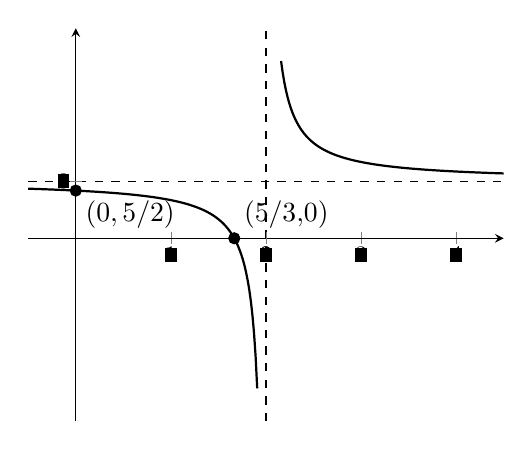
\begin{tikzpicture}
        \begin{axis}[restrict y to domain=-10:10, extra y ticks={3}, extra x ticks={2},
            samples=300, ytick=\empty]
          \addplot[domain=-0.5:4.5] {3+1/(x-2)};
          \addplot[closed] coordinates {(0,2.5) (5/3,0)};
          \node[below right] at (0, 2.5) {$(0, 5/2)$};
          \node[above right] at (5/3, 0) {$(5/3,0)$};
        \end{axis}
      \end{tikzpicture}
    \end{solution}

  \item
    \begin{problem}[0.75in]
      Are your answers to (a) and (b) consistent with each other? 
    \end{problem}

    \begin{solution}
      Yes. If we draw the tangent line to the graph at $x=1$, it has a negative slope.

      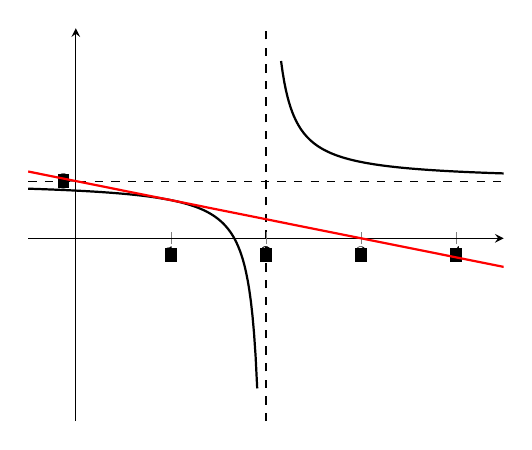
\begin{tikzpicture}
        \begin{axis}[restrict y to domain=-10:10, extra y ticks={3}, extra x ticks={2},
            samples=300, ytick=\empty]
          \addplot[domain=-0.5:4.5] {3+1/(x-2)};
          \addplot[domain=-0.5:4.5, red] {-(x-1)+2};
        \end{axis}
      \end{tikzpicture}
    \end{solution}

  \item
    \begin{problem}[\vfill]
      Put the following quantities in increasing order. Justify your ordering. 
      \[ f'(3) \qquad f'(4) \qquad f'(5) \]
    \end{problem}

    \begin{solution}
      Thinking about the slopes of the tangent lines to the graph at $x=3$, $x=4$,
      and $x=5$, we can see that they are all negative. As $x$ increases from $3$ to $5$,
      the tangent lines become less steep, so the slopes become less negative. Therefore
      \[f'(3) < f'(4) < f'(5).\]
    \end{solution}
  \end{enumerate}

\end{enumerate}
\end{document}
